\documentclass[tikz]{standalone}
\usepackage{pgfplots}
\usepgfplotslibrary{groupplots}
\pgfplotsset{width=12cm, height=9cm, compat=1.18}
\usepackage{tikz}
\usepackage{circledsteps}
\usepackage{gensymb}
\usepackage{amsmath}
\usepackage[outline]{contour}
\contournumber{64}% default is 16, star form uses 32
\contourlength{.12em}% default is 0.03em
\usetikzlibrary {arrows.meta} 
\usetikzlibrary{decorations.pathreplacing, calligraphy}

\begin{document}
	
	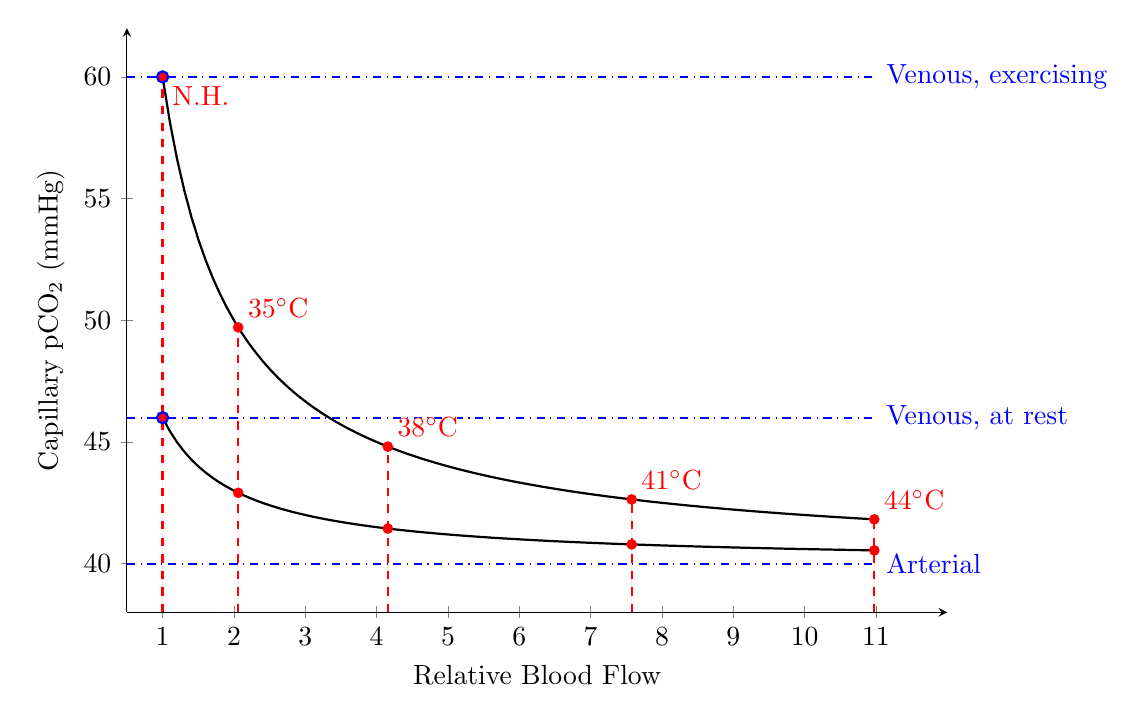
\begin{tikzpicture}
		\begin{axis}[
			axis lines = left,
			xlabel = Relative Blood Flow,
			y axis line style = {black},
			ylabel style = {black},
			ylabel = Capillary pCO$_2$ (mmHg),
			xmin=0.5, xmax=12,
			ymin=38, ymax=62,
			xtick={1,2,3,4,5,6,7,8,9,10,11},
			% xlabel style = {at={(ticklabel cs:.98)}, anchor=south},
			% ytick=\empty,
			%clip mode=individual,
			clip=false,
			]
			\tikzstyle bfnode=[circle,fill=blue,minimum size=5pt, inner sep=0pt];
			\tikzstyle barrow=[red, very thick, {Stealth[length=3mm]}-{Stealth[length=3mm]}];
			%
			\draw[blue, dashdotted, thick] (0.5,40) -- (11,40) node[anchor=west] {Arterial};
			\draw[blue, dashdotted, thick] (0.5,60) -- (11,60) node[anchor=west] {Venous, exercising};
			\draw[blue, dashdotted, thick] (0.5,46) -- (11,46) node[anchor=west] {Venous, at rest};
			\addplot[
			thick,
			domain = 1:11,
			samples = 100,
			] {1/x*46 + (x-1)/x*40};
			\addplot[
			thick,
			domain = 1:11,
			samples = 100,
			] {1/x*60 + (x-1)/x*40};
			%\addplot[fill=black, mark=*, mark size=1.5pt] (1, 46);
			%\addplot[fill=black, mark=*, mark size=1.5pt] (1, 60);
			\pgfplotsinvokeforeach{1,2.0604,4.1570,7.5752,10.9769}{
				\draw[dashed, red, thick, fill=red] (#1,38) -- (#1,{1/#1*46 + (#1-1)/#1*40}) -- (#1,{1/#1*60 + (#1-1)/#1*40});
				\draw[red, thick, fill=red] (#1,{1/#1*46 + (#1-1)/#1*40}) circle[radius=1.5pt];
				\draw[red, thick, fill=red] (#1,{1/#1*60 + (#1-1)/#1*40}) circle[radius=1.5pt];
			};
		\draw (1,60) node[red, anchor=north west]{N.H.};
		\draw (2.0604,49.70685304) node[red, anchor=south west]{35{\degree}C};
		\draw (4.1570,44.8111619) node[red, anchor=south west]{\contour{white}{38{\degree}C}};
		\draw (7.57521,42.64019432) node[red, anchor=south west]{41{\degree}C};
		\draw (10.9769,41.82200804) node[red, anchor=south west]{44{\degree}C};
		% blue circles
		\draw[blue, thick] (1,60) circle[radius=2pt];
		\draw[blue, thick] (1,46) circle[radius=2pt];
		\end{axis}	
	\end{tikzpicture}
	%
\end{document}